% !TeX spellcheck=en_GB
\documentclass[a4paper,10pt]{article}
%\usepackage{setspace}
\usepackage{parskip}
\usepackage[T1]{fontenc}
\usepackage[english]{babel}
\usepackage{csquotes}
\usepackage{amsmath}
\usepackage{tikz}
\usetikzlibrary{calc}
\usepackage[shortlabels]{enumitem}
\usepackage{subcaption}
\usepackage{graphicx}
\usepackage{geometry}
\usepackage{hyperref}
\geometry{margin=2.5cm}

% Platzhalter fuer spaeter einzufuegende Abbildungen
\newcommand{\Platzhalter}[2][8cm]{%
  \begin{center}
  \fbox{\begin{minipage}[c][#1][c]{0.7\textwidth}
    \centering \itshape #2
  \end{minipage}}
  \end{center}
}

\title{Crafting manual for a Doktorhut (AGAG Kaiserslautern)}
\author{\footnotesize Adapted from:\\\footnotesize\url{https://jura.uni-koeln.de/fileadmin/institute/versicherungsrecht/Promotionen/Doktorhut.pdf}}
\date{10 August 2026}

%\setstretch{0.9}
\setlist{itemsep=0pt, topsep=3pt}

\begin{document}
	\maketitle
	
	\section*{General description of the hat}
	
	The hat consists of two parts (see also Figure~\ref{fig:side}): A cylinder of circumference $ C $, diameter $ D=C/\pi $ and height $ H $, and a top square of side length $ S_1 $. The circumference $ C $ coincides with the circumference of the PhD student's hat, which should be measured. We have cardboard rings of different sizes to help with this. All other dimensions of the hat that are used below ($ H $, $ D $, $ S_1 $, $ S_2 $, $ T $, $ H' $, $ C' $) can be computed from $ C $ using \texttt{Doktorhut\_Dimensions.ods}, and they are also explained there.
	
	\begin{figure}[htb]
		% ---------- Colours ----------
\colorlet{hat-colour}{black!20}
\colorlet{cardboard-colour}{brown!20}
\colorlet{circle-colour}{black}
\colorlet{teeth-colour}{black!40}
\begin{subfigure}{0.3\textwidth}
	\centering\begin{tikzpicture}
		\def\SquareLength{2} % Half the with of the top
		\def\CylLength{1} % Half the width of the cylinder
		\def\CylHeigth{2} % Height of the cylinder
		% Shift of the dimensions arrows <->
		\def\ShiftX{0.2}
		\def\ShiftY{0.3}
		% Position of coordinates:
		% ULL - UL - UR - URR
		%       LL - LR
		\coordinate (ULL) at (-\SquareLength, 0);
		\coordinate (UL) at (-\CylLength, 0);
		\coordinate (UR) at (\CylLength, 0);
		\coordinate (URR) at (\SquareLength, 0);
		\coordinate (LL) at (-\CylLength, -\CylHeigth);
		\coordinate (LR) at (\CylLength, -\CylHeigth);
		% Draw hat
		\draw[thick, fill=hat-colour] (UL) -- (UR) -- (LR) -- (LL) -- cycle;
		\draw[line width=1] (ULL) -- (URR);
		% Draw dimensioning
		\draw[<->] ($ (ULL) + (0,\ShiftY) $) -- ($ (URR) + (0,\ShiftY) $) node[midway, above]{$ S_1 $};
		\draw[<->] ($ (LL) + (0,-\ShiftY) $) -- ($ (LR) + (0,-\ShiftY) $) node[midway, below]{$ D $};
		\draw[<->, overlay] ($ (URR) + (\ShiftX, 0) $) -- ++(0, -\CylHeigth) node[midway, right]{$ H $};
	\end{tikzpicture}
	\caption{The finished hat from the side.}
	\label{fig:side}
\end{subfigure}%
% ---------- Parameters of the following two drawings ----------
\def\OuterSquareLength{2}% Side length of the outer square
\def\CircleRadius{0.55}% Radius of the cylinder circle
\def\nTeeth{20}% Number of teeth
\def\ToothRadius{0.35} % Radius of the (invisible) inner circle on which all ends of teeth lie
% ---------- Derived parameters of the drawings ----------
\pgfmathsetmacro{\ToothAngle}{360/\nTeeth}
\pgfmathsetmacro{\LastToothAngle}{360-\ToothAngle}
% ---------- Shifts for dimensioning ----------
\def\OuterSquareDimYShift{0.1}
\def\InnerSquareDimXShift{0.05}
\def\InnerSquareDimYShift{-0.05}
% ---------- Labels ----------
\def\OuterSquareLabel{$ S_2 $}
\def\InnerSquareLabel{$ S_1 $}
\def\DiameterLabel{$ D $}
\begin{subfigure}{0.3\textwidth}%
	\centering\begin{tikzpicture}[x=2cm,y=2cm]
		\coordinate (circle-mid) at (\OuterSquareLength/2, \OuterSquareLength/2);
		
		% Outer square
		\draw[fill=hat-colour] (0,0) rectangle (\OuterSquareLength, \OuterSquareLength);
		% Inner square
		\draw[fill=cardboard-colour] (\OuterSquareLength/2, 0) -- (\OuterSquareLength, \OuterSquareLength/2) -- (\OuterSquareLength/2, \OuterSquareLength) -- (0, \OuterSquareLength/2) -- cycle;
		
		% ---------- Dimensioning ----------
		% Outer square
		\draw[<->, shift={(0,-\OuterSquareDimYShift)}] (0,0) -- (\OuterSquareLength,0) node[midway,below]{\OuterSquareLabel};
		% Inner square
		\draw[<->, shift={(\InnerSquareDimXShift, \InnerSquareDimYShift)}] (\OuterSquareLength/2, 0) -- (\OuterSquareLength, \OuterSquareLength/2) node[midway, below right]{\InnerSquareLabel};
	\end{tikzpicture}%
	\caption{Gluing~\ref{black-square} onto~\ref{cardboard}.}%
	\label{fig:squares}
\end{subfigure}%
\begin{subfigure}{0.33\textwidth}
	\centering\begin{tikzpicture}[x=2cm,y=2cm]%[line width=0.8pt]
		\coordinate (circle-mid) at (\OuterSquareLength/2, \OuterSquareLength/2);
		
		% Inner square
		\draw[fill=hat-colour] (\OuterSquareLength/2, 0) -- (\OuterSquareLength, \OuterSquareLength/2) -- (\OuterSquareLength/2, \OuterSquareLength) -- (0, \OuterSquareLength/2) -- cycle;
		% Teeth
		\pgfmathsetmacro{\LastNumber}{\nTeeth-1}
		\foreach \x in {0, 1, ..., \LastNumber}{
			\pgfmathsetmacro{\StartAngle}{\x*\ToothAngle}
			\pgfmathsetmacro{\MidAngle}{(\x+0.5)*\ToothAngle}
			\pgfmathsetmacro{\EndAngle}{(\x+1)*\ToothAngle}
			
			\draw[fill=teeth-colour, shift=(circle-mid)] (\StartAngle:\CircleRadius) arc[start angle=\StartAngle, end angle=\EndAngle, radius=\CircleRadius] -- (\MidAngle:\ToothRadius) -- cycle;
		}
		% Circle
		\draw[thick, circle-colour] (circle-mid) circle[radius=\CircleRadius];
		
		% ---------- Dimensioning ----------
		% Inner square
		\draw[<->, shift={(\InnerSquareDimXShift, \InnerSquareDimYShift)}] (\OuterSquareLength/2, 0) -- (\OuterSquareLength, \OuterSquareLength/2) node[midway, below right]{\InnerSquareLabel};
		% Diameter
		\draw[<->, shift=(circle-mid)] (-\CircleRadius,0) -- (\CircleRadius,0) node[midway,below]{\DiameterLabel};
	\end{tikzpicture}%
	\caption{The finished hat from below.}
	\label{fig:below}
\end{subfigure}

		\caption{Illustrations.}
	\end{figure}
	
%	\section*{Measurements to take}
%	
%	The circumference $ C $ of the hat of the PhD student (usually $ 60 \text{cm} \pm 3 \text{cm} $) should be measured. We have cardboard rings of different sizes to help with this. All other dimensions ($ H $, $ D $, $ S_1 $, $ S_2 $, $ T $, $ H' $, $ C' $) can be computed from this value using \texttt{Doktorhut\_Dimensions.ods}, though the PhD student might have a different preference for the height $ H $ of the hat.
	

	
	\section*{Required Materials}
	
	\begin{enumerate}[(1)]
		\item Thick black paper (we normally use \enquote{Fotokarton 50x70 schwarz} from McPaper, the thickness is probably 300$ \text{g}/\text{cm}^2 $):
		\begin{enumerate}[label=(1.\alph*)]
			\item\label{black-cyl} A rectangle of size $ C' \times H' $ for the cylinder.
			\item\label{black-square} A square of size $ S_2 \times S_2 $ for the top.
		\end{enumerate}
		
		\item\label{cardboard} A thick cardboard square of size $ S_1 \times S_1 $ around which black cardboard will be wrapped. This square will not be visible in the end, so it can be ugly: Cardboard from a large package works. It is important that the cardboard is thick enough, like $ 0.5\text{cm} $.
		
		\item A cord for the tassel (\enquote{Quaste}).
		
		\item Glue stick (liquid glue leaves visible traces).
		
		\item Ruler, scissors and, if possible, a Geodreieck.
	\end{enumerate}
	
	\newpage
	
	\section*{Top}
	
	The top consists of the thick cardboard square~\ref{cardboard}, around which the black paper~\ref{black-square} is wrapped.
	
	\begin{enumerate}[(a)]
		\item\label{top:first-step} Put the thick cardboard square in the center of black square, as in Figure~\ref{fig:squares}. Fold the overlapping four black triangles around the cardboard to check that the four triangles together completely cover the backside of the cardboard.
		
		\item If the black paper does not cover the backside of the cardboard: Cut off a bit of the cardboard to reduce its side length by 1mm (make sure that the edge of the cardboard remains straight!) and return to step~\ref{top:first-step}.
		
		\item Put glue on the middle of~\ref{black-square} and glue it on top of~\ref{cardboard}.
		
		\item Put glue on the four black triangles which overlap the cardboard, fold them around the cardboard, and glue them onto its backside. The cardboard should now be completely covered by black paper.
		
		\item Put a heavy object onto the top to ensure that it does not deform while the glue dries.
	\end{enumerate}
	
	Thought: Possibly it is easier to construct the top like this: \\
	\url{https://gws2.de/doktorhut-zum-aufsetzen-basteln-anleitung/}
	
	\section*{Cylinder}
	
	Cut out the shape in Figure~\ref{fig:cylinder} from the black rectangle~\ref{black-cyl}. (The angles in the figure are merely approximations and do not have to be considered.) This shape consists of the following parts:
	\begin{itemize}
		\item A big rectangle of size $ C \times H $ which will ultimately form the cylinder.
		
		\item A flap below the big rectangle which increases stability.
		
		\item A gluing flap on the left of the rectangle.
		
		\item Teeth above the rectangle which will be used to glue together the cylinder and the top. The precise number of teeth, as well as their width $ T $, depends on the head circumference $ C $.
	\end{itemize}
	
	Now glue the left flap onto the right-hand side of the big rectangle to obtain a cylinder.
	
	\begin{figure}[htb]
		\centering\documentclass[tikz,border=10pt]{standalone}
\usepackage{tikz}
\usetikzlibrary{arrows.meta,calc}

\begin{document}
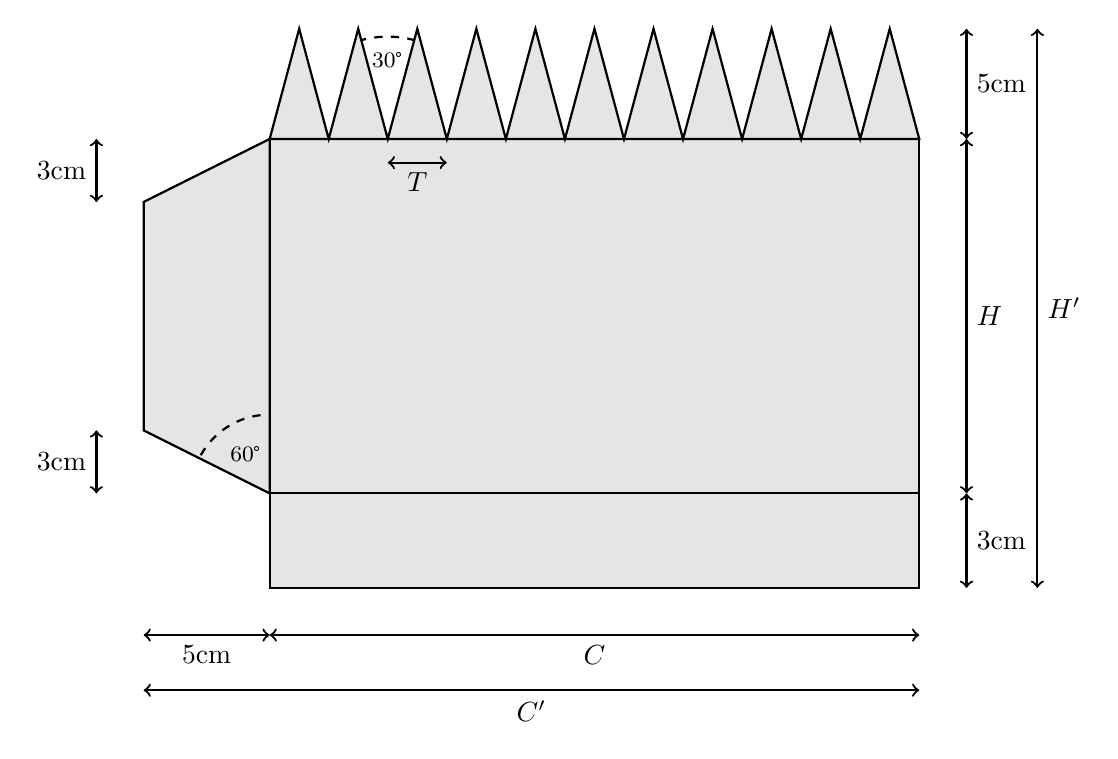
\begin{tikzpicture}[line width=0.8pt]

% ---------- Parameters of the drawing ----------
% Dimensions of the drawing
\def\CylHeight{4.5}          % Height H of the cylinder
\def\LowerFlapHeight{1.2}          % Height of the lower flap
\def\nTeeth{11}       % Total number of teeth
\def\ToothHeight{1.4}           % Height of a tooth
\def\ToothWidth{0.75}  % Width of a tooth
\def\LeftFlapWidth{1.6}          % Width of the left flap
\def\LeftFlapHeightShorten{0.8}  % Amount by which the height of the left flap is shortened relative to the height of the cylinder

% Distance to dimensioning labels
\def\LowerDimensioningDistanceShort{0.6} % Vertical distance between the drawing and the dimensioning on the bottom
\def\LowerDimensioningDistanceLong{1.3}
\def\RightDimensioningDistanceShort{0.6} % Horizontal distance between the drawing and the dimensioning on the right
\def\RightDimensioningDistanceLong{1.5}
\def\UpperDimensioningDistance{0.3}
\def\LeftDimensioningDistance{0.6}

% Angle label on the left flap
\def\LeftFlapAngleRadius{1}
\def\LeftFlapAngleLabelXShift{-0.3}
\def\LeftFlapAngleLabelYShift{0.5}

% Angle label on the teeth
\def\ToothAngleRadius{1.3}
\def\ToothAngleLabelYShift{1}

% ---------- Derived parameters of the drawing ----------
\pgfmathsetmacro{\RectangleWidth}{\nTeeth*\ToothWidth} % Circumference C of the head of the PhD student
\pgfmathsetmacro{\LeftFlapAngle}{atan(\LeftFlapWidth / \LeftFlapHeightShorten)}

% ---------- Labels of the drawing ----------
\def\ToothWidthLabel{$ T $}
\def\LeftFlapWidthLabel{5cm}
\def\RectangleWidthLabel{$ C $}
\def\TotalWidthLabel{$ C' $};

\def\ToothHeightLabel{5cm}
\def\CylHeightLabel{$ H $}
\def\LowerFlapHeightLabel{3cm}
\def\TotalHeightLabel{$ H' $}
\def\LeftFlapHeightShortenLabel{3cm}

\def\LeftFlapAngleLabel{60°}
\def\ToothAngleLabel{30°}

% ---------- Colours ----------
\colorlet{fillcolor}{black!10}
\colorlet{helplinecolor}{gray}


% (0,0) coordinate = upper left corner of rectangle

% ---------- Basic rectangle ----------
\draw[fill=fillcolor] (0,0) rectangle (\RectangleWidth,-\CylHeight);

% ---------- Lower flap ----------
\draw[fill=fillcolor] (0,-\CylHeight) rectangle (\RectangleWidth, -\CylHeight-\LowerFlapHeight);
% Trennlinie zwischen H-Bereich und 3cm-Streifen
\draw (0,-\CylHeight) -- (\RectangleWidth,-\CylHeight);

% ---------- Left flap + angle ----------
\begin{scope}
	\draw[fill=fillcolor] (-\LeftFlapWidth,-\LeftFlapHeightShorten) -- (0,0) -- (0,-\CylHeight) -- ++(-\LeftFlapWidth, \LeftFlapHeightShorten) -- cycle;
	% Draw the arc around the desired angle by clipping a full circle to the path of the left flap
	\path[clip] (-\LeftFlapWidth,-\LeftFlapHeightShorten) -- (0,0) -- (0,-\CylHeight) -- ++(-\LeftFlapWidth, \LeftFlapHeightShorten) -- cycle;
	\draw[dashed] (0,-\CylHeight) circle[radius=\LeftFlapAngleRadius];
	\node[font=\footnotesize] at (\LeftFlapAngleLabelXShift, -\CylHeight+\LeftFlapAngleLabelYShift){\LeftFlapAngleLabel};
\end{scope}


% ---------- Teeth on top ----------
\draw[fill=fillcolor]
	(0,0)
	\foreach \i in {1,...,\nTeeth} {
	  -- ++(\ToothWidth/2,\ToothHeight) -- ++(\ToothWidth/2,-\ToothHeight)
	}
	-- cycle;

% ---------- Dimensioning: Width ----------
\begin{scope}
	% Left flap-
	\draw[<->] (0,-\CylHeight-\LowerFlapHeight-\LowerDimensioningDistanceShort) -- ++(-\LeftFlapWidth,0) node[midway,below]{\LeftFlapWidthLabel};
	% Rectangle
	\draw[<->] (0,-\CylHeight-\LowerFlapHeight-\LowerDimensioningDistanceShort) -- ++(\RectangleWidth,0) node[midway,below]{\RectangleWidthLabel};
	% Total width
	\draw[<->] (-\LeftFlapWidth,-\CylHeight-\LowerFlapHeight-\LowerDimensioningDistanceLong) -- ++(\LeftFlapWidth+\RectangleWidth, 0) node[midway,below]{\TotalWidthLabel};
\end{scope}

% ---------- Dimensioning: Height, right ----------
\begin{scope}
	% Teeth
	\draw[<->] (\RectangleWidth+\RightDimensioningDistanceShort,0)-- ++(0,\ToothHeight) node[midway,right]{\ToothHeightLabel};
	% Cylinder
	\draw[<->] (\RectangleWidth+\RightDimensioningDistanceShort,0) -- ++(0,-\CylHeight) node[midway,right]{\CylHeightLabel};
	% Lower flap
	\draw[<->] (\RectangleWidth+\RightDimensioningDistanceShort,-\CylHeight) -- ++(0,-\LowerFlapHeight) node[midway,right]{\LowerFlapHeightLabel};
	% Total
	\draw[<->] (\RectangleWidth+\RightDimensioningDistanceLong,\ToothHeight)-- ++(0,-\ToothHeight-\CylHeight-\LowerFlapHeight) node[midway,right]{\TotalHeightLabel};
\end{scope}

% ---------- Dimensioning: Height, left ----------
\foreach \y\sign in {0/-, -\CylHeight/+}{
	\draw[<->] (-\LeftFlapWidth-\LeftDimensioningDistance, \y) -- ++(0, \sign\LeftFlapHeightShorten) node[midway,left]{\LeftFlapHeightShortenLabel};
}

% ---------- Dimensioning: Teeth ----------
\draw[<->] (2*\ToothWidth, -\UpperDimensioningDistance) -- ++(\ToothWidth,0) node[midway,below]{\ToothWidthLabel};

% ---------- Angle on teeth ----------
\begin{scope}
	\coordinate (base) at (2*\ToothWidth,0);
	\path[clip] (base) -- +(-\ToothWidth/2, \ToothHeight) -- +(\ToothWidth/2, \ToothHeight) -- cycle;
	\draw[dashed] (base) circle[radius=\ToothAngleRadius];
	
	\node[font=\footnotesize] at ($ (base) + (0,\ToothAngleLabelYShift) $){\ToothAngleLabel};
\end{scope}


\end{tikzpicture}
\end{document}

		\caption{The shape to cut out from~\ref{black-cyl} for the cylinder.}
		\label{fig:cylinder}
	\end{figure}

	\section*{Combining top and cylinder}
	
	\begin{enumerate}[(a)]
		\item Fold the teeth to the inner side of the cylinder and glue them to the top.
		
		\item Put a heavy object into the cylinder to ensure that it does not deform while the glue dries.
	\end{enumerate}

	\section*{Tassel (Quaste)}
	
	To be written.


	\section*{Decoration}
	
	The following ideas for decoration can often be adapted to the individual PhD student:
	\begin{itemize}
		\item Photos (of the working group, of the student giving a talk, \dots).
		
		\item Flags (of the student's home country, of the country that they will move to, of a country that they visited often during their PhD, of their home town or some union, \dots).
		
		\item A personalised Lego figure of the PhD student.
		
		\item Handcrafted items (from paper, cardboard, wool, household items, \dots). Ideas for themes:
		\begin{itemize}
			\item The PhD student's hobbies and preferences. This may include sports, food, pets/animals, music, games/books/media they like, \dots
			
			\item Illustrations, diagrams, formulas or numbers from the PhD thesis (drawn on the hat, crafted from material, printed out, \dots).
			
			\item Mathematical objects that appear in their PhD thesis: E.g. a presentation for a group, \dots
			
			\item Puns relating to the topic of the thesis (e.g. \enquote{tropical geometry} $\to$ a tropical landscape, \enquote{Hecke algebras} $\to$ a hedge).
			
			\item Landmarks of countries that are important to the student.
			
			\item Folklore relating to the student's country of origin. Be careful not to be insensitive.
		\end{itemize}
		
		\item Possibly friends and family of the PhD student can be contacted for ideas.
	\end{itemize}
	
	You can find examples of previous hats here: \url{https://seafile.rlp.net/d/4d68de46e89b4933b0e0/}

\end{document}
